\subsection{Episode 2: In the Tiki, Tiki, Tiki, Tiki, Tiki Room}

The year is 6653 CC (Church Calendar). In their search for the Stone of Un'thala, the group set off Southwards from Vathos Boundary following the directions given to them by the hunter, Gerard.\medskip

After a day’s travelling the group settle down for the night with Kolo and Pilch taking the first watch. The tension and hatred between the two is palpable and they stare intently at each other. Pilch is briefly distracted, which gives Kolo the chance to disappear. As Pilch desperately searches for his goblin nemesis, Kolo takes the opportunity to attempt to relieve a sleeping Otoria of some of her gold. As he reaches into her pocket Otoria awakes and deals a deadly blow to the goblin, knocking him unconscious.\medskip

Otoria throws the bundle of goblin into his tent, awaking his sister in the process, who mistakenly believes it is her turn to perform lookout duties. She sets down opposite Pilch and resumes the goblin-human stare off. Pilch inquires about Exme’s “gun”, but is not prepared for the onslaught of technical information that Exme is only too glad to discuss. The conversation ends with Pilch being none the wiser, embarrassed by his own vast ignorance. When Exme returns to her tent Kolo has vanished.\medskip

The group push on towards their goal. After some time they arrive at a large skull shaped ice temple that lies across a perilous looking bridge. Exme refuses to enter without her brother and stubbornly resists the efforts of Riphard to carry her along. Otoria takes charge and heads into the temple.\medskip

As the group enter the temple they find themselves in a large spherical chamber, and have their first meeting with the dreaded TikkiTukks™: a race of small bear like creatures with fearsome, culturally insensitive masks. Battle ensues, with the goblins arriving to witness the felling of the final enemy. An investigation of the stone plinth at the centre of the chamber shows that the stone is missing. The goblins remove some masks from the fallen enemies revealing their ghastly faces with sharp, pointed teeth.\medskip

The reassembled group head deeper into the temple in search of the stone. Otoria takes a moment to collect some herbs being cultivated by the TikkiTukks™.\medskip

Kolo unlocks a locked door, which reveals a room full of small boxes that contain some treasure which the group splits up.** Pilch** attempts to reclaim some of the money that he had "misplaced" in the previous session, shamefully accusing the goblins of thievery. Otoria throws him an azure gem to appease him. As the gold is shared out Riphard warns the goblins: “Next time you want your fair share, join the battle at the right time”.\medskip

The goblins attempt to trick another room of TikkiTukks™ by donning masks. Kolo is able to speak in the TikkiTukk™ language. Exme, not knowing of her brothers ability, attempts a bold deception which ultimately backfires when the two are brought to their knees by the devastating attacks from a room full of TikkiTukks™. The group defeat the TikkiTukks™ and enjoy a short rest to recuperate.\medskip

As they continue to explore,** Kolo** pulls Exme back, warning her of a strange tangle of silk threads that hang in a corridor. The group is set upon by a giant spider.** Pilch** is able to set fire to the webbing that covers the walls and ceiling, which keeps the spider at bay, but also traps Otoria on the wrong side of the flames as she delivers her swordy brand of justice. After a short struggle the spider explodes in a mass of ichor.\medskip

Riphard is having gun troubles.\medskip

Continuing on, Riphard activates an ancient trap that fires darts at the group. However, the goblins are not affected since they are of a similar height to the TikkiTukks™; the darts passing harmlessly over them.\medskip

The group manage to fight a large room full of TikkiTukks™, slaughtering their leader (who begins the battle with the glorious war cry ‘tikki tukk doumo arigatou tikki tukk’ ) and claiming his glorious mask as their own. Even with their Tikkitactics and Packtics they are no match for the group.\medskip

Riphard is still having gun troubles.\medskip

The impotent Riphard falls in battle. Kolo kindly revives him whilst pocketing 5 gp, going easy on the man he has no real qualms with yet.\medskip

Further battles ensue. Otaria falls. In a desperate attempt to revive her Exme accidentally punches her in the face, pushing her one step closer to death. Kolo looks on in dismay. Riphard is able to revive her, and the two share a tender moment as he lays his hands on her for “a little too long”.\medskip

Freshly rested the group find a corridor of doors. In full synchronisation, the crew knock down 4 doors only to find, to Kolo’s dismay, more doors inside: “More DOORS. TRICKSY, TRICKSY!!”\medskip

Riphard takes a moment to explore and comes across a fresh water well. He drinks from it and feels the benefits of its cool water, but already feeling 100\% despite the recent battles, does not fully appreciate the benefits the refreshing beverage provides, and so does not share this wisdom with the group.\medskip

The noise of the group knocking/cutting in half doors causes the TikkiTukks™ to bear down upon them.\medskip

Riphard is still still having gun troubles. Exasperated, he makes one last effort and is finally rewarded for his patience and persistence, destroying what once was a young TikkiTukk's™ face in one well placed and devastating shot.\medskip

The group leave one TikkiTukk™ alive to interrogate and help them locate the stone. Whilst passed out, the TikkiTukk™ is tied up and hung upside down. The two goblins don their masks and get ready to intimidate him. Kolo leads the interrogation. The TikkiTukk™ is keen not to die and quickly reveals that the stone is held in the chief’s room. In exchange for the location of the stone of Un'thala, Kolo promises the TikkiTukk™ that he can be the new TikkiTukk™ chief.** Pilch** is also offered as a “sweetener”.\medskip

Kolo is keen to take the prisoner along, but Otoria cryptically states that she is to “have her way with him”. Pilch, greedy for the prisoner’s vitality through his curse attempts to end its life. Otoria is able to block the first blow, but misses the second, which slices open the TikkiTukk’s™ throat. In a cool rage Otoria pins Pilch up against the wall with her large sword and warns him: “I have to work with you, we have shared goals. But you will not do that again”. Pilch is filled with an intense terror at these words.\medskip

The group collect themselves and prepare to head to the chief’s lair to collect their prize

\begin{center}
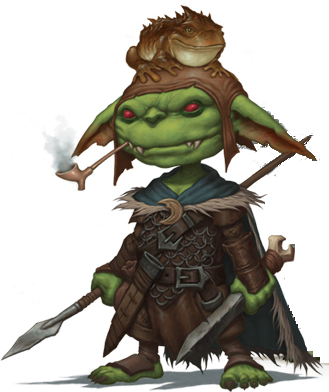
\includegraphics[width=80mm]{./content/img/kolo2.png}
\begin{figure}[h]
\end{figure}
\end{center}

\clearpage

